\chapter{Clock System}

\paragraph*{}
In diesem Abschnitt wird das Clock-System behandelt. Es ermöglicht den Prozessor und andere Bestandteile des Chips mit unterschiedlichen Taktraten zu betreiben. Durch betreiben des Controllers mit geringerem Takt kann Strom gespart werden, und so mit eine längere Laufzeit erreicht werden. Außerdem wird die Rechenleistung des Controllers für den jeweiligen Anwendungszweck optimiert. Auch hat der Takt Einfluss auf viele Peripheriegeräte wie zum Beispiel die Timer.

\section*{Aufgabe 5}

\paragraph*{}
Für die Lösung dieser und der nachfolgenden Aufgabe, war es nicht nötig ein Programm zu schreiben, wir konnten die Werte der erforderlichen Register über den Debugger direkt modifizieren. Gleichzeit maßen wir mit einem angeschlossenen Oszilloskop die aktuelle Frequenz des MCLK-Taktes, die über P5.5 nach außen geführt wird, wenn die P5SEL und P5DIR entsprechend gesetzt sind.

\paragraph*{}
Unsere Ergebnisse finden sich in nachfolgender Tabelle: \\

\begin{tabular}{ p{4cm} | c | p{4cm} }\hline \hline
Clocksrv & DIVM-Bits & Frequenz \\ \hline
DCOCLK & 00 & 776,5 Khz \\ \cline{2-3}
DCOCLK & 01 & 388 Khz \\ \cline{2-3}
DCOCLK & 10 & 194,1 Khz \\ \cline{2-3}
DCOCLK & 11 & 97 Khz \\ \hline
XT2CLK & 00 & 7,37 Mhz \\ \hline
LFXT1CLK & 00 & 32,77 Khz \\ \hline
\end{tabular}

\paragraph*{}
Mit durch setzen des DCOR-Bits auf 1 wird ein externer Widerstand angeschlossen. Dies führt nach unseren Beobachtungen zu einem stabileren Takt. Mit dem DIVM-Bits wird der Divisor gesteuert. Er ermöglicht es Bruchteile der eigentlichen Taktquelle zu erhalten. 

\section*{Aufgabe 6}

\paragraph*{}
Durch unsere Messung konnten wir einen linearen Zusammenhang zwischen Strom und der Frequenz des MCLK-Taktes feststellen. Dies erscheint logisch unter der Annahme das ein Schaltvorgang konstant viel Strom benötigt, unabhängig davon wie lang der Zustand anschließend gehalten werden muss.

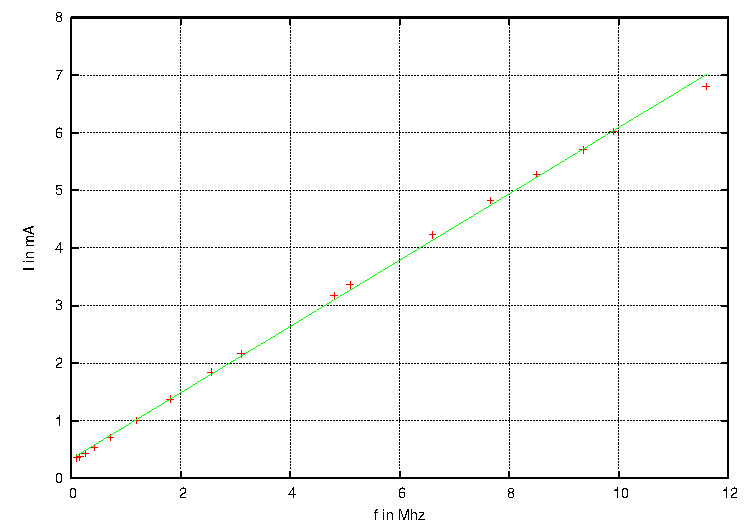
\includegraphics[width=\textwidth]{graphs/vfgraph.pdf}


\section*{Aufgabe 7}

\paragraph*{}
Um die gewünschten Einstellung zu treffen nutzen wir die Register {\em DCOCTL},{\em BCSCTL1} und {\em BCSCTL2}. Die genauen nötigen Einstellung ermittelten wir vorher nach dem trail-and-error Prinzip.

\lstinputlisting[caption=aufgabe7.c]{src/aufgabe7.c}

\paragraph*{}
Anschließend konnten wir am angeschlossenen Ampermeter folgende Werte ermitteln: \\

\begin{tabular}{ c | c | c }\hline \hline
Frequenz & Stromverbrauch & Laufzeit mit 1100 mAh Batterie \\ \hline
4,096 kHz & 0,376 mA & 2926 h (ca. 122 Tage) \\ \hline
7,3728 MHz & 4,635 mA & 273 h (ca. 10 Tage) \\ \hline
\end{tabular}

\section*{Aufgabe 8}

\paragraph*{}
Da wir direkt auf den Prozessor zu greifen, und wir keine weiteren Programmflüsse auf dem Prozessor laufen haben, ist die Ausführungszeit eines Befehls gegeben als das Reziprok der Prozessorfrequenz. Unter der Voraussetzung das die Operation in einem Takt abgearbeitet werden kann. 

\lstinputlisting[caption=aufgabe8.c]{src/aufgabe8.c}

\paragraph*{}
Für unsere spezielle Aufgabe muss beachtet werden, das wir als Messergebnis eine Frequenz über zwei Zustandsänderungen erhalten. Mittels des obigen Programms gelang es uns folgende Werte zu ermitteln: \\

\begin{tabular}{ c | c | c | c}\hline \hline
MCLK-Takt & gemessene Frequenz & errechnete Zeit \\ \hline
7,37 Mhz & 263,43 Khz & $ 3,796 * 10^{-6} $ s  \\ \hline
32,77 Khz & 1,17 Khz & $ 8,547 * 10^{-4} $ s  \\ \hline
\end{tabular}

\paragraph*{}
Die Frequenz des Prozessors ist wesentlich höher als die am Pin anliegende, da zwei Durchläufe der Schleife eine Periode am Pin entsprechenden. Hinzu kommt das nicht nur zum Umschalten sondern auch für das Abarbeiten der Schleifen Maschinenoperationen gebraucht werden. 

